\section{Controle de Baixo Nível}
\label{sec:baixo_nivel}

O controle de baixo nível do VIDA tem como objetivo garantir o acompanhamento das referências de velocidade longitudinal e ângulo de esterçamento estabelecidas pelo sistema de navegação ou pela operação manual. Para isso, são empregadas duas malhas de controle, responsáveis por compensar os desvios entre as referências solicitadas e as grandezas medidas pelos sensores embarcados. As ações de controle resultantes são convertidas em comandos para os sistemas de tração, esterçamento e frenagem, respeitando as limitações operacionais e os mecanismos de segurança da plataforma. As estratégias de controle e suas respectivas implementações são apresentadas nas subseções seguintes.

\subsection{Controle de Esterçamento}
\label{subsec:controle_esterçamento}

O controle de esterçamento tem como finalidade regular o ângulo das rodas dianteiras a partir de uma referência estabelecida pelo sistema de navegação ou pela operação manual. Para isso, foi implementado um controlador proporcional-integral-derivativo (PID) discreto, executado a uma frequência nominal de 200~Hz. A realimentação é fornecida pelo sensor LVDT, cuja medição de deslocamento linear é convertida em ângulo de esterçamento por meio de uma relação de calibração.

A lei de controle pode ser expressa por:

\begin{equation}
u_{\delta}(t) =
K_p e_{\delta}(t)
+ K_i \int_0^t e_{\delta}(\tau)\,d\tau
- K_d \dot{\delta}_{m,f}(t)
\end{equation}

em que $u_{\delta}$ representa o sinal de controle, $K_p$, $K_i$ e $K_d$ são os ganhos proporcional, integral e derivativo, respectivamente, e $e_{\delta}$ corresponde à diferença entre o ângulo de referência e o ângulo medido. O termo $\dot{\delta}_{m,f}$ representa a taxa de variação filtrada do ângulo de esterçamento medido.

Uma particularidade dessa implementação é a aplicação da ação derivativa sobre a medição, em vez de diretamente sobre o erro de controle. Essa estratégia evita que alterações abruptas da referência produzam picos na parcela derivativa, fenômeno conhecido como \textit{derivative kick}, contribuindo para uma resposta mais suave do sistema de acionamento \citep{AstromHagglund2006}. 

Antes de ser utilizada pela malha de controle, a referência de esterçamento é submetida a restrições de amplitude e de taxa de variação. O ângulo solicitado é limitado à faixa de $\pm20^\circ$, enquanto sua variação máxima é estabelecida em $40^\circ/\mathrm{s}$. Essas restrições reduzem solicitações bruscas ao mecanismo de direção e contribuem para manter o comando dentro da faixa operacional definida para o veículo.

Além das ações PID, o controlador incorpora recursos destinados a melhorar o comportamento do sistema diante das características do acionamento eletromecânico. Entre eles estão uma zona morta com histerese, a compensação do atrito estático e mecanismos de integração condicionada e anti-windup. A zona morta com histerese contribui para evitar acionamentos sucessivos próximos à condição de equilíbrio, enquanto a compensação do atrito estático auxilia no início do movimento do mecanismo. Os mecanismos associados à ação integral, por sua vez, limitam seu acúmulo em condições nas quais o esforço de controle não pode ser integralmente aplicado.

O firmware também considera restrições associadas aos limites físicos de esterçamento. Embora a referência de operação seja limitada a $\pm20^\circ$, o mecanismo possui um limite de segurança de $\pm25^\circ$. Dessa forma, são impedidos comandos que possam ampliar o esterçamento quando o ângulo medido já se encontra além da faixa permitida.

A Figura~\ref{fig:controle_esterçamento} apresenta a estrutura da malha fechada de controle de esterçamento, reunindo os elementos descritos anteriormente. O diagrama destaca o processamento da referência, a atuação do controlador PID, os mecanismos de compensação e limitação dos comandos, o acionamento do motor de direção e a realimentação fornecida pelo sensor LVDT.

% -----------------------------------------------------------
% FIGURA: DIAGRAMA DA MALHA FECHADA DE ESTERÇAMENTO
% Manter o caminho da imagem já utilizado no seu projeto.
% -----------------------------------------------------------
\begin{figure}[htb]
    \centering
    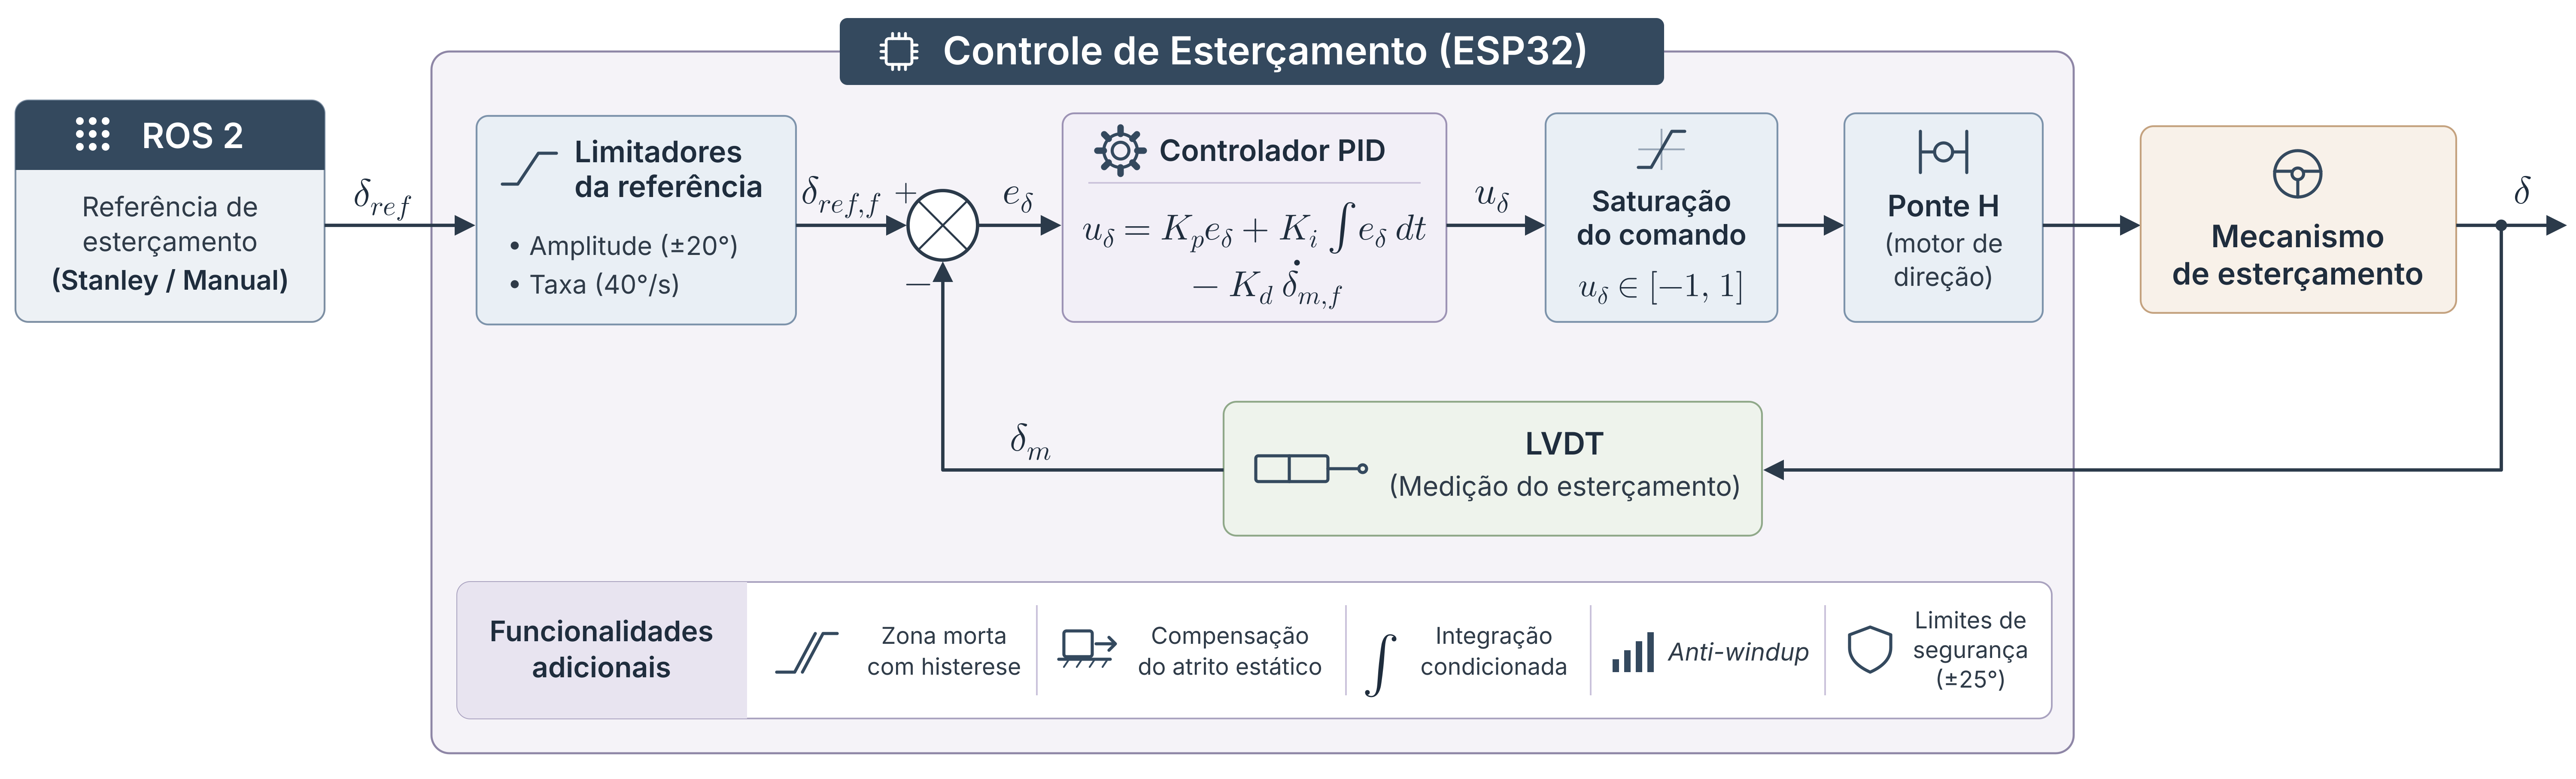
\includegraphics[width=\columnwidth]{Imagens/Malha de controle esterçamento.png}
    \caption{Diagrama da malha fechada de controle do ângulo de esterçamento. Fonte: Elaborado pelo autor.}
    \label{fig:controle_esterçamento}
\end{figure}

Os ganhos do controlador foram inicialmente ajustados com o auxílio de simulações e posteriormente refinados por meio de ensaios experimentais na plataforma VIDA. A Tabela~\ref{tab:parametros_esterçamento} apresenta os ganhos e os limites operacionais adotados na configuração utilizada durante a validação experimental.

\begin{table}[htb]
    \centering
    \caption{Parâmetros do controlador de esterçamento.}
    \label{tab:parametros_esterçamento}
    \begin{tabular}{lc}
        \hline
        \textbf{Parâmetro} & \textbf{Valor} \\
        \hline
        Ganho proporcional ($K_p$) & 0,05 \\
        Ganho integral ($K_i$) & 0,10 \\
        Ganho derivativo ($K_d$) & 0,002 \\
        Limite da referência & $\pm20^\circ$ \\
        Limite de segurança & $\pm25^\circ$ \\
        Taxa máxima da referência & $40^\circ/\mathrm{s}$ \\
        Frequência de controle & 200~Hz \\
        \hline
    \end{tabular}
\end{table}

\subsection{Controle de Velocidade Longitudinal}
\label{subsec:controle_velocidade}

Para regular a velocidade longitudinal do VIDA, foi adotada uma estratégia de controle em malha fechada baseada em um controlador proporcional-integral (PI) discreto, executado a uma frequência nominal de 200~Hz. O controlador determina o esforço necessário para acompanhar a velocidade de referência, utilizando as medições dos encoders como realimentação. A ação de controle resultante é utilizada para coordenar os sistemas de tração e frenagem, permitindo tanto a aceleração quanto a desaceleração do veículo.

A realimentação utiliza a média das velocidades medidas pelos encoders instalados nas rodas dianteiras, que não são diretamente acionadas pelo sistema de tração. Essa configuração reduz a influência de eventuais perdas de aderência da roda traseira motriz sobre a medição da velocidade longitudinal. A velocidade utilizada pelo controlador é calculada por:

\begin{equation}
v_m = \frac{v_{de} + v_{dd}}{2}
\end{equation}

em que $v_m$ representa a velocidade longitudinal medida, enquanto $v_{de}$ e $v_{dd}$ correspondem às velocidades medidas nas rodas dianteiras esquerda e direita, respectivamente. 

A partir da velocidade medida, o controlador determina o erro em relação à referência recebida e calcula o esforço necessário para sua correção. A lei de controle PI pode ser expressa por:

\begin{equation}
u_v(t) = K_p e_v(t) + K_i \int_0^t e_v(\tau)\,d\tau
\end{equation}

em que $u_v$ representa o esforço de controle longitudinal normalizado, $K_p$ e $K_i$ são os ganhos proporcional e integral, respectivamente, e $e_v$ corresponde à diferença entre a velocidade de referência e a velocidade medida. Valores positivos de $u_v$ são utilizados para gerar comandos de tração, enquanto valores negativos são tratados pela lógica de desaceleração e frenagem.

Antes de ser aplicada ao controlador, a referência de velocidade é submetida a restrições de amplitude e de taxa de variação. A velocidade máxima permitida é de $2,5~\mathrm{m/s}$, enquanto rampas de aceleração e desaceleração estabelecem transições graduais entre diferentes condições de movimento. A aceleração padrão é definida em $0,4~\mathrm{m/s^2}$, podendo ser alterada se encaminhada pelo ROS2 junto com a referência de velociade. A desaceleração máxima é limitada a $1,0~\mathrm{m/s^2}$. 

Para evitar o acúmulo excessivo da ação integral em condições de saturação, o controlador incorpora um mecanismo de \textit{anti-windup} baseado em integração condicionada. Além disso, o estado integral é reinicializado quando o sistema não possui permissão de movimento, evitando que erros acumulados durante períodos de desabilitação produzam comandos inadequados após uma nova habilitação.

O esforço de controle calculado é encaminhado a uma lógica de acionamento responsável pela coordenação dos sistemas de tração e frenagem. Para esforços positivos, é gerado um comando destinado ao motor de tração, incluindo a compensação da zona morta de acionamento. Para esforços negativos, a estratégia permite inicialmente a desaceleração em roda livre e, quando necessário, o acionamento progressivo do freio mecânico por meio do servomotor.

A condição de parada recebe tratamento específico. Quando a referência de velocidade atinge valores próximos de zero, a ação PI é desabilitada e o sistema passa a comandar o freio mecânico, mantendo-o aplicado durante a condição de parada. Essa estratégia evita acionamentos sucessivos do sistema de tração provocados por pequenas oscilações na velocidade medida. Adicionalmente, durante a operação manual, o operador pode solicitar a aplicação imediata do freio por meio do gatilho do gamepad, independentemente do esforço calculado pelo controlador PI.

A Figura~\ref{fig:controle_velocidade} apresenta a estrutura da malha fechada de controle longitudinal, reunindo os elementos descritos anteriormente. O diagrama destaca o processamento da referência, a atuação do controlador PI, os mecanismos de limitação e compensação, a distribuição dos comandos entre os sistemas de tração e frenagem e a realimentação fornecida pelos encoders.

% -----------------------------------------------------------
% FIGURA: DIAGRAMA DA MALHA FECHADA DE VELOCIDADE
% Manter o caminho original da imagem no seu projeto.
% -----------------------------------------------------------
\begin{figure}[htb]
    \centering
    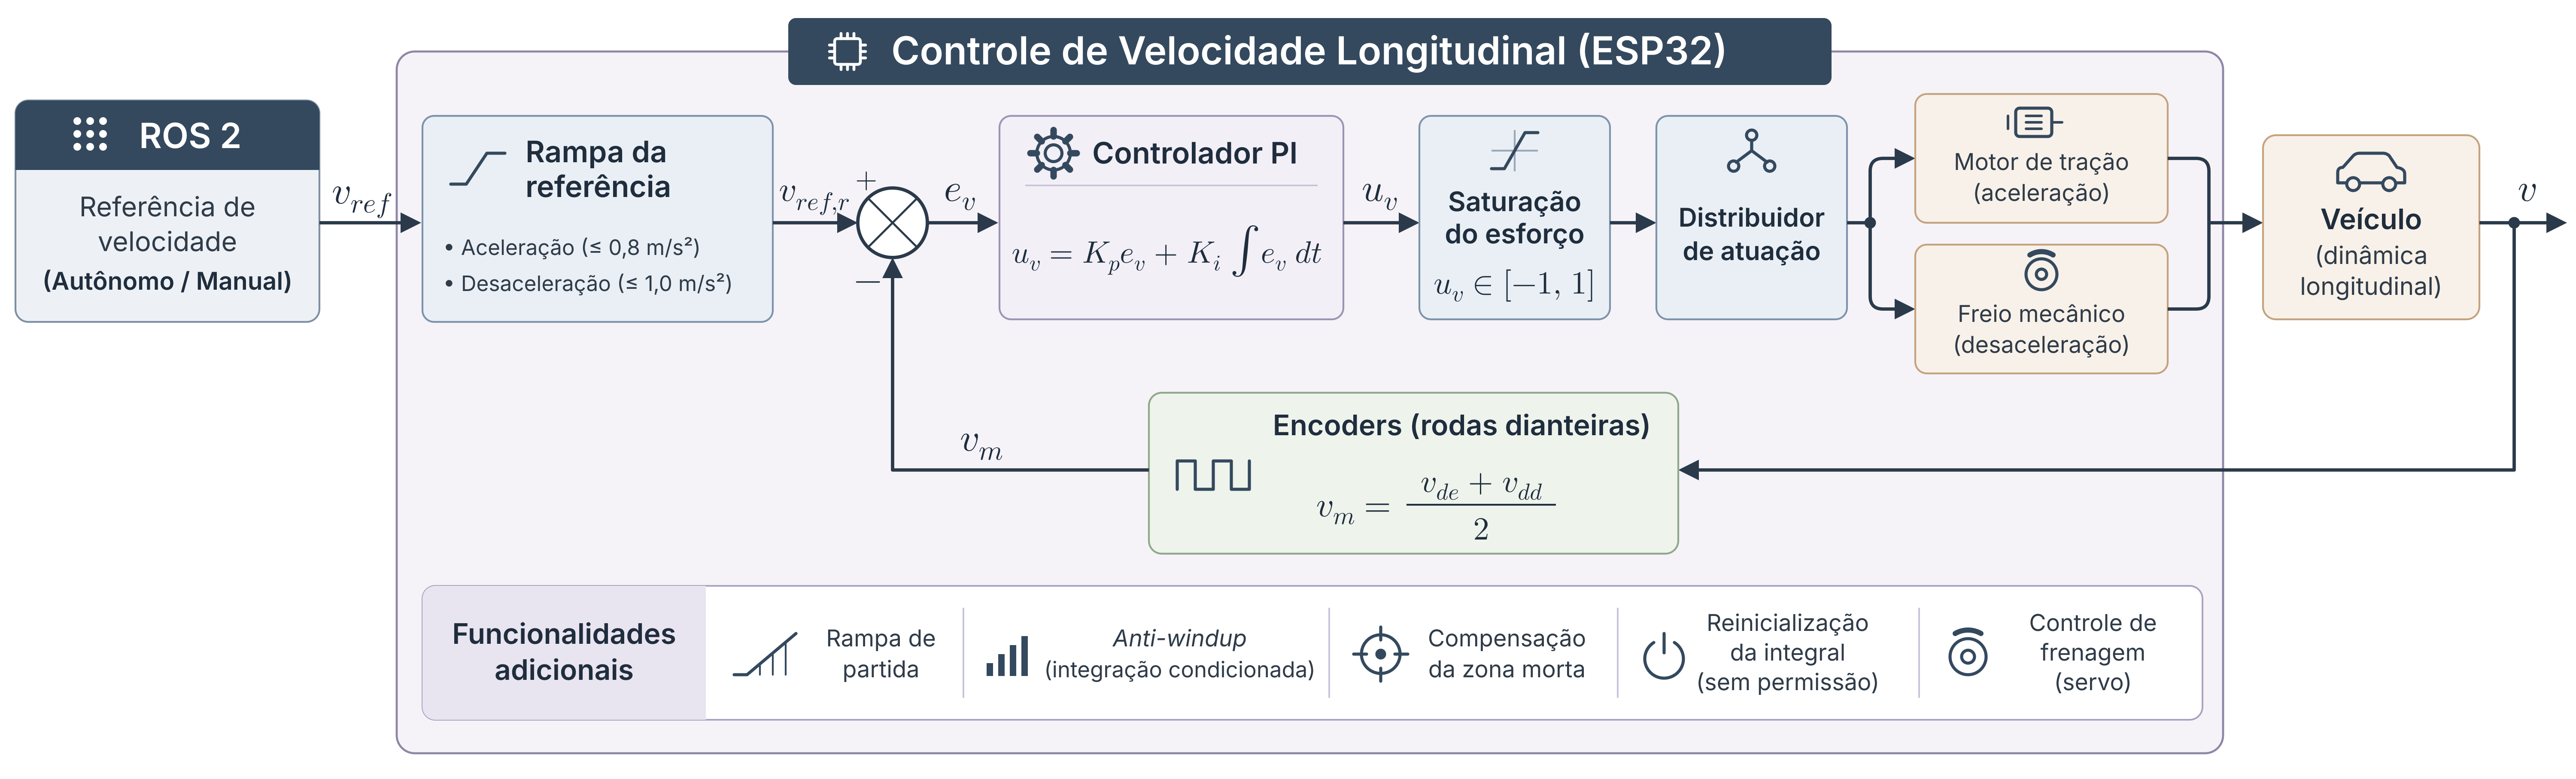
\includegraphics[width=\columnwidth]{Imagens/Malha de controle longitudinal.png}
    \caption{Diagrama da malha fechada de controle de velocidade longitudinal. Fonte: Elaborado pelo autor.}
    \label{fig:controle_velocidade}
\end{figure}

Os ganhos do controlador foram inicialmente ajustados com o auxílio de simulações e posteriormente refinados por meio de ensaios experimentais na plataforma VIDA. A Tabela~\ref{tab:parametros_controle_velocidade} apresenta os ganhos e os limites operacionais adotados na configuração utilizada durante a validação experimental.

\begin{table}[htb]
    \centering
    \caption{Parâmetros do controle de velocidade longitudinal.}
    \label{tab:parametros_controle_velocidade}
    \begin{tabular}{lc}
        \hline
        \textbf{Parâmetro} & \textbf{Valor} \\
        \hline
        Ganho proporcional ($K_p$) & 0,10 \\
        Ganho integral ($K_i$) & 0,025 \\
        Frequência de controle & 200~Hz \\
        Velocidade máxima & $2,5~\mathrm{m/s}$ \\
        Aceleração padrão & $0,4~\mathrm{m/s^2}$ \\
        Aceleração máxima & $0,8~\mathrm{m/s^2}$ \\
        Desaceleração máxima & $1,0~\mathrm{m/s^2}$ \\
        \hline
    \end{tabular}
\end{table}